\section{Experiments}

In this chapter we describe the evaluation setup,

In this section we show:
- Description of the evaluation setup, how long the models trained, which hardware was used,
which networks were used. Any specifics of the traning procedure. Sizes of the replay tables,
learning rates.

\subsection{Evaluation setup}

We evaluate our architecture on the subset of VizDoom and Atari tasks and compare it with the
performance of DQN. All experiments are performed on Microsoft Azure NC6 instances, with NVidia K80
video card and 6 cores of Intel Xeon Processor E5-2690 v3. We use the neural network architecture
described in \cite{NatureDQN}, that consists of convolutional layer with 32 filters of size $8
\times 8$ with stride 4, followed by convolutional layer with 64 filters of size $4 \times 4$ with
stride 2, followed by a convolutional layer with 64 filters of size $3 \times 3$ with stride 1,
followed by a fully connected layer with 512 hidden units. All four hidden layers were followed by
a rectifier nonlinearity. The input of the network comes from state space and,
the output of the network consists of $\abs{\Actions}$ units that represent a value of Q-function
for all actions in the input state $Q(s, \cdot)$.
All experiments use discount factor $\gamma = 0.99$ and Adam optimizer.

\subsection{Hyperparameters sensitivity analysis}

To validate that our learning algorithm is robust to hyperparameters choice, we conduct a sweep
over the grid of parameters on VizDoom level DoomDefendCenter and present the obtained learning
curves.

- Explanation why the algorithms perform as they do. Study on how hyperparameters influence
the performance both in terms of training speed and efficiency.

\begin{figure}[h!]
\caption{Parameter sweep for DoomDefendCenter environment}
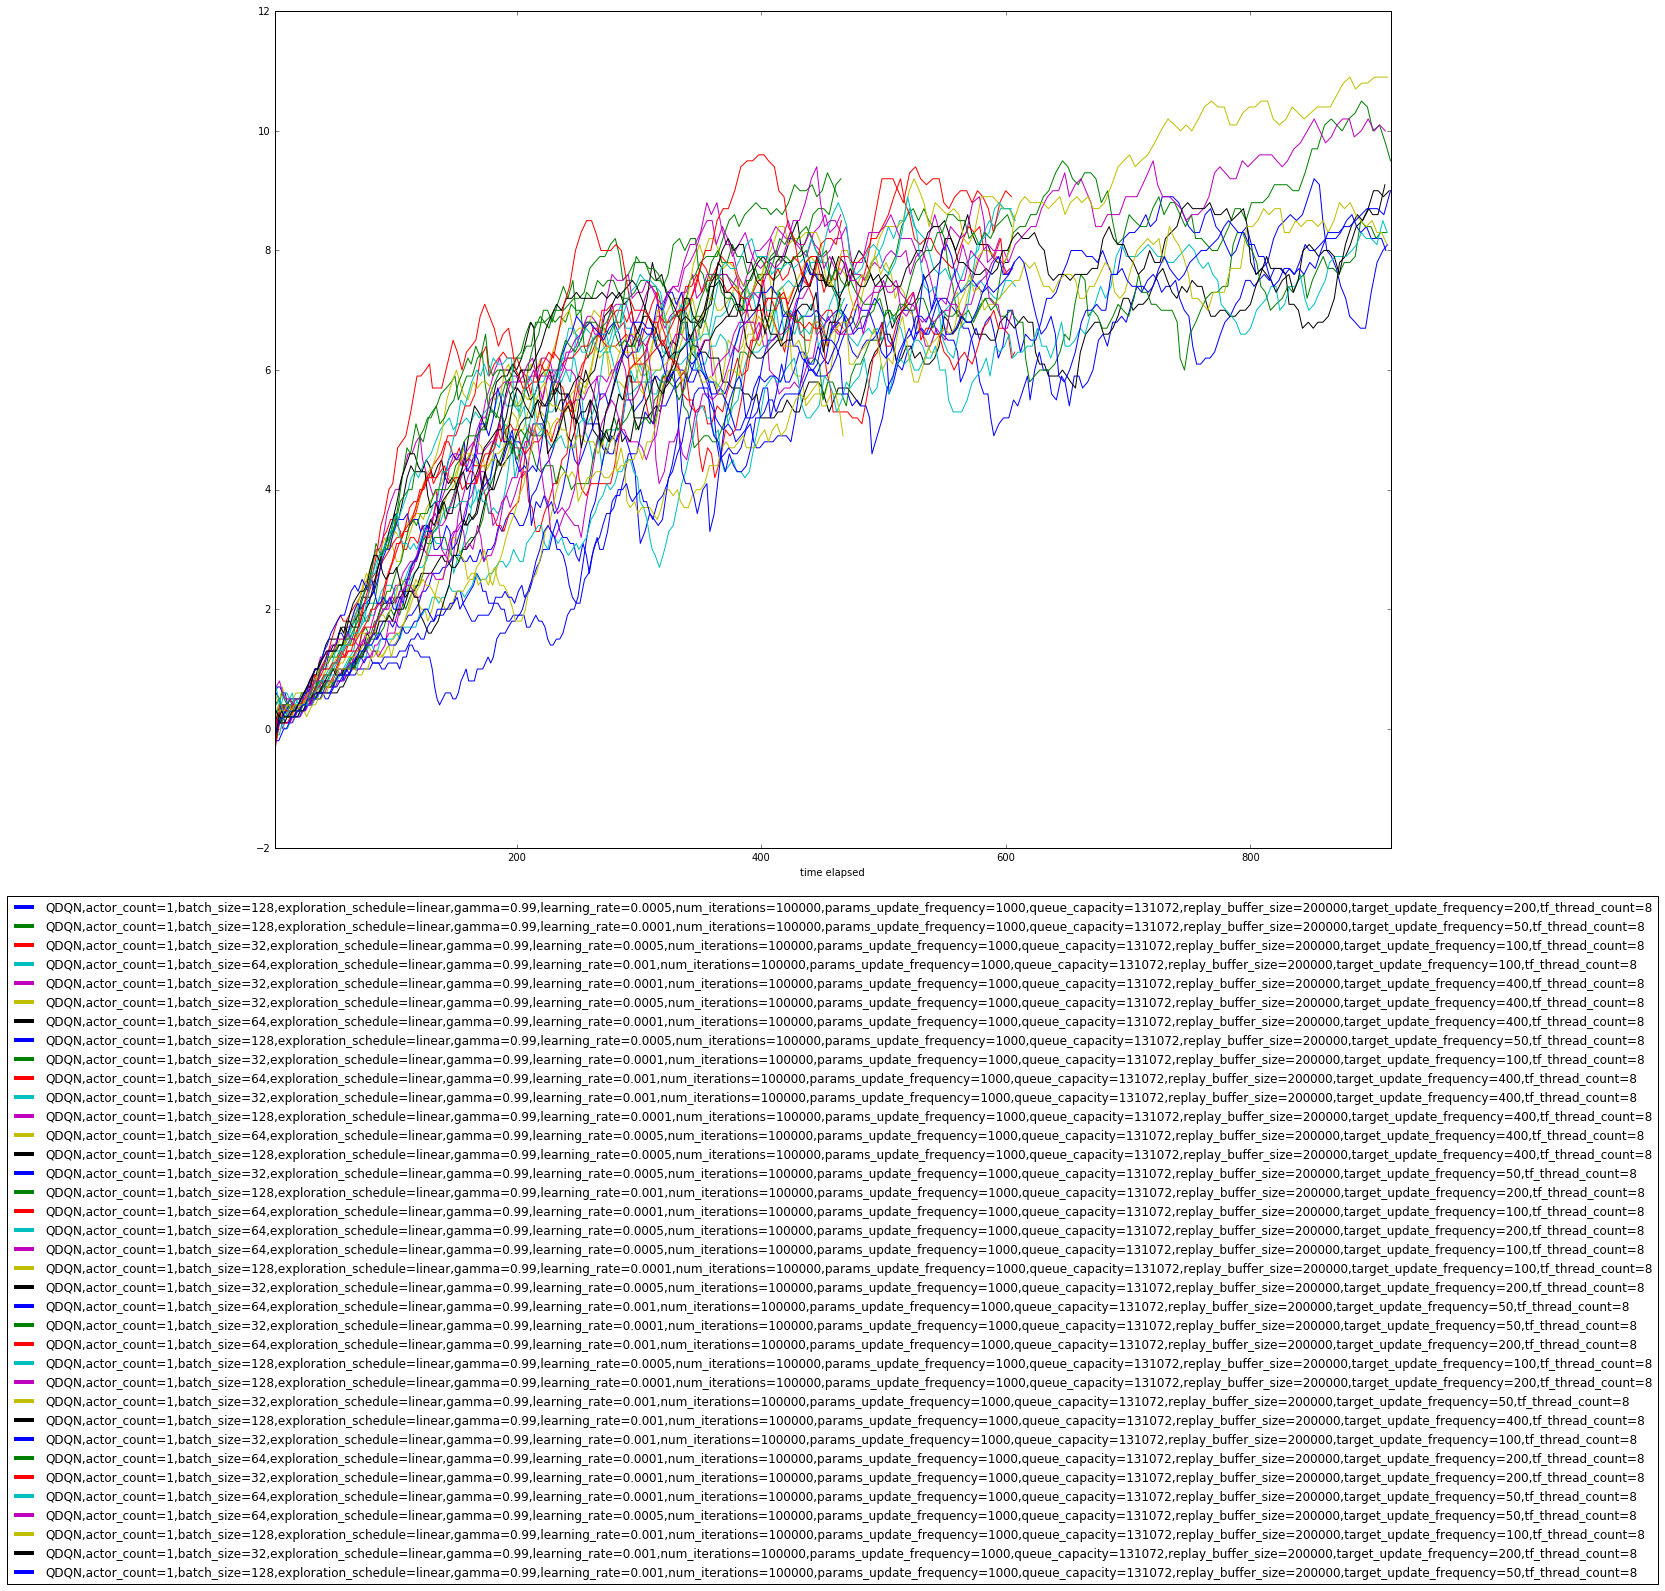
\includegraphics[width=\textwidth]{doom_sweep}
\end{figure}

\subsection{Training speed comparison}

\paragraph{Doom}
As a preprocessing step, we rescale images to $80 \times 80$ and transform them from RGB to greyscale.
We also introduce a frame skip of size 4, meaning that each agent action is repeated for 4 consecutive frames.
We use the replay table of size $50000$, and anneal exploration ratio $\eps$ linearly from 1 to 0.02
over the first $1/4$ of training iterations. We use learning rate of $1e-4$.

- Graphs of DQN, DecoupledDQN performance on 3 VizDoom Gym levels.

\paragraph{Atari}
We use the same input preprocessing as in \cite{NatureDQN}, involving rescaling images to $84
\times 84$ and turning them from RGB into greyscale, and also introducing a frame skip of size 4.
We use the replay table of size $200000$, and anneal exploration ratio $\eps$ linearly from 1 to 0.02
over the first $1/4$ of training iterations. We use learning rate of $1e-4$.

- Graphs of DQN, DecoupledDQN performance on 3 Atari games.

- Explanation what is on the graph, how we made the measurements robust to the noise (choosing top 5
from several random seeds).

- How the methods perform in terms of wall time/sample efficiency.
